
\section{Introduction to DataStudio}
\label{datastudio}

\textbf{Quick Reference Guide}

%Shown below is the quick reference guide for DataStudio.

\vspace{0.3cm}
{\par\centering \resizebox*{0.90\textwidth}{!}{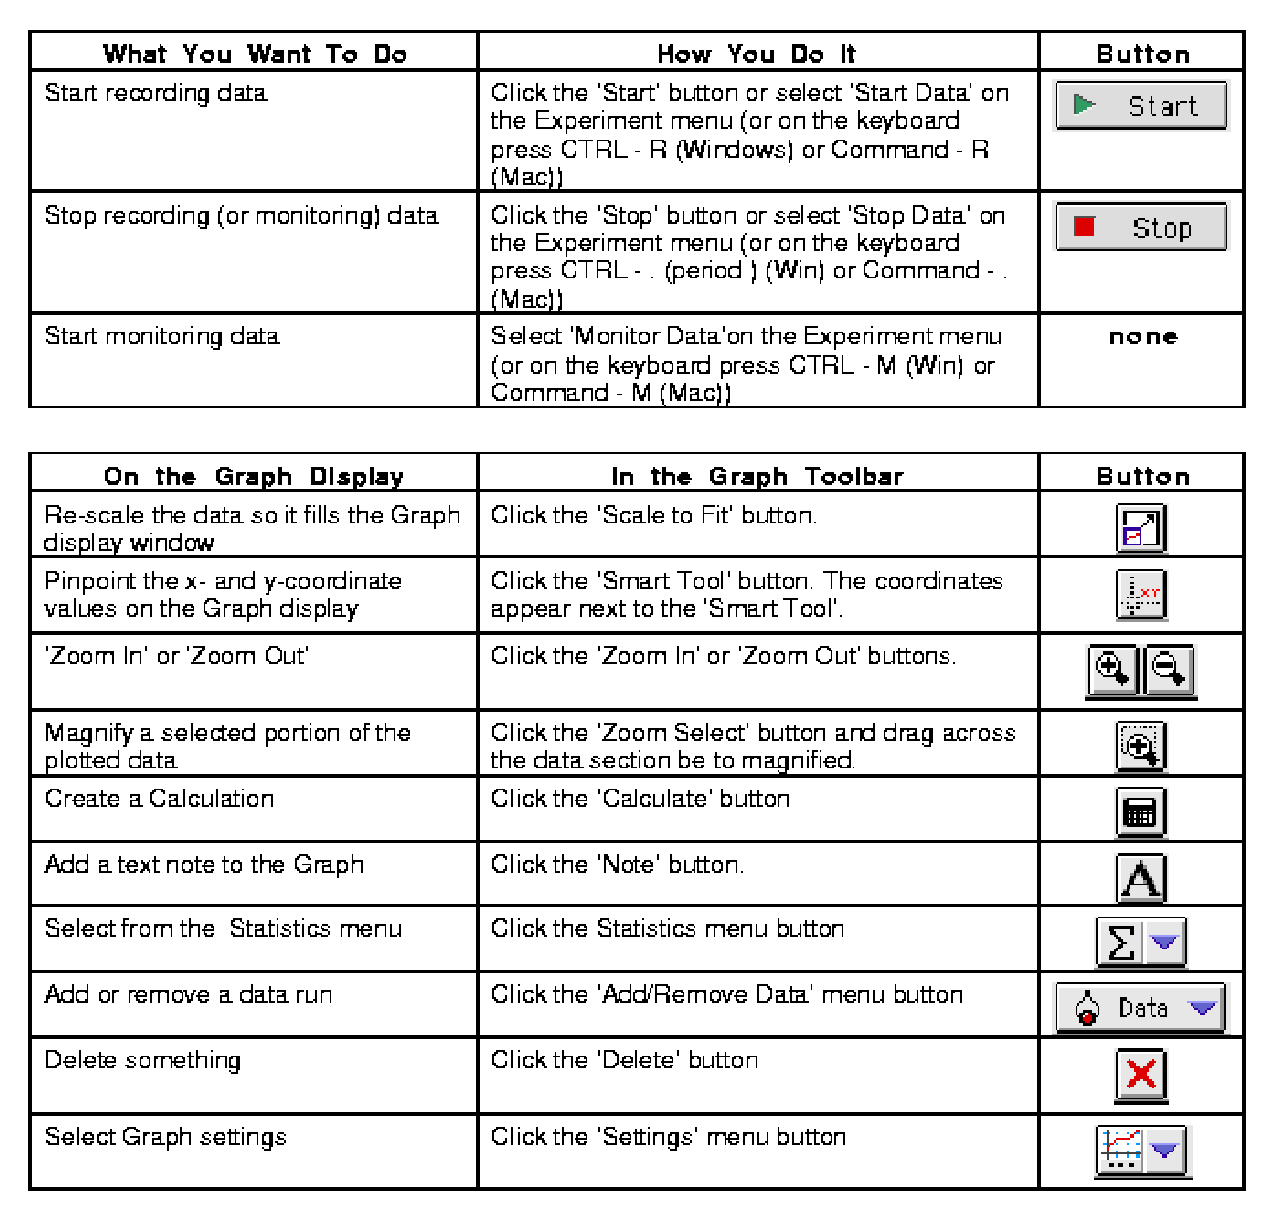
\includegraphics{../../131/StudentGuideModule1/appendices/datastudio/datastudio_fig1.eps}} \par}
\vspace{0.3cm}

\textbf{Selecting a Section of Data}

\begin{enumerate}
\item To select a data section, hold the mouse button down and move the cursor to
draw a rectangle around the data of interest. The data in the region of interest
will be highlighted.
\item To unselect the data, click anywhere in the graph window.
\end{enumerate}
\textbf{Fitting a Section of Data}

\begin{enumerate}
\item Select the section of data to be fitted.
\item Click on the \textbf{Fit} button on the Graph Toolbar and select a mathematical
model. The results of the fit will be displayed on the graph.
\item To remove the fit, click the \textbf{Fit} button and select the checked function
type.
\end{enumerate}


\pagebreak[2]
\textbf{Finding the Area Under a Curve}

\begin{enumerate}
\item Use the \textbf{Zoom Select} button on the Graph Toolbar to zoom in around the
region of interest in the graph. See the quick reference guide above for instructions.
\item Select the section of data that you want to integrate under.
\item Click the \textbf{Statistics} button on the Graph Toolbar and select \textbf{Area}.
The results of the integration will be displayed on the graph.
\item To undo the integration, click on the \textbf{Statistics} button and select
\textbf{Area}.
\end{enumerate}

\textbf{Calibrating Force Sensors}

\begin{enumerate}
\item Connect force sensor to Pasco interface (in port ``A'').

\item Open whatever software application you will be using in the current experiment.

\item Click ``Setup''.

\item Click ``Calibrate Sensors''.

\vspace{0.1in}
\hspace{-0.2in}FOR HORIZONTAL USE:

\item Set force sensor on track, and with no force applied to the sensor, press TARE button on side of the sensor. This sets the sensor to zero. Then set 1st calibration point to 0 newtons, press upper ``Read from sensor'' button.

\item While holding sensor stationary (with your hand), hang 200g from sensor over a pulley at end of track, as in Figure 2 of Experiment 13. Set 2nd calibration point to 1.96 newtons, press lower ``Read from sensor'' button.

\item Click ``OK''. Force sensor is now calibrated for the rest of your experiment. Close ``Calibrate Sensors'' window, close ``Setup'' window.

\item While still holding the force sensor still, press ``Start''. Graph should now show a reading of 1.96 N. Press ``Stop''.

\item Try hanging a different mass from the force sensor (over the pulley); press ``Start'' and check that it is reading correctly.

\vspace{0.1in}
\hspace{-0.2in}FOR VERTICAL USE:

\setcounter{enumi}{4}

\item Holding sensor vertically (with hook down and no force applied to it), press TARE button on side of the sensor. This sets the sensor to zero. Then set 1st calibration point to 0 newtons, press upper ``Read from sensor'' button.

\item Hang 200 g from sensor, set 2nd calibration point to 1.96 newtons, press lower ``Read from sensor'' button.

\item Click ``OK''. Force sensor is now calibrated for the rest of your experiment. Close ``Calibrate Sensors'' window, close ``Setup'' window.

\item While still holding the force sensor still, press ``Start''. Graph should now show a reading of 1.96 N. Press ``Stop''.

\item Try hanging a different mass from the force sensor; press ``Start'' and check that it is reading correctly.
\end{enumerate}
